\documentclass[class=jsarticle, crop=false, dvipdfmx, fleqn]{standalone}
\input{/Users/User/Documents/University/report_template/preamble/preamble}
\begin{document}
\section*{宿題2}

MNISTを用いた手書き数字分類を行う。
各画像は\(784\ (= \num{28 x 28})\)次元ベクトルとして扱い,
各数字は正規分布に従うと仮定する。
正規分布のパラメータをMNIST学習データで推定し,
そのパラメータにより識別関数を決定してテストデータを識別する。

識別関数は,
\begin{itemize}
    \item Case 1: \(\bm{\Sigma}_i = \sigma^2 \bm{I}\)
    \item Case 2: \(\bm{\Sigma}_i = \bm{\sigma}\)
    \item Case 3: \(\bm{\Sigma}_i = \text{arbitrary}\)
\end{itemize}
の3ケースについて考える。
式(\ref{eq:log_prob_y_given_x})を用いれば,
ある\(\bm{x}\)について,
対数事後確率\(\log(p(y|\bm{x}))\)がそれぞれのラベル\(y\)について求まる。
この値が最大となるものを予測値とすればよい。



\subsection*{プログラム}

プログラムの本体は\pageref{listing:assignment2}ページの
listing \ref{listing:assignment2}に示す。
共分散行列が正則でなかったため,
その逆行列として,ムーア・ペンローズの疑似逆行列を用いた。
また,Case 3において,
共分散行列の行列式が全てのラベルで0となったが,
計算の都合上,行列式の関わる項(\(\log(\det(\bm{\Sigma}))\))は無視した。

以下に含まれる関数の簡単な説明を記載する。

\begin{itemize}
    \item load\_data \\
        MNISTのデータを読み込み,
        train用の画像とラベル,
        test用の画像とラベルの計4つの配列を返す関数。
    \item get\_statistics \\
        画像データの統計量を取る。
        ここで統計量とは,あるラベルに属する画像データの数・その全体に対する割合(事前確率)・平均・共分散行列である。
    \item train \\
        各Caseで用いる共分散行列を求め,
        対数事後確率を求めるのに用いる関数(log\_prob\_n)を決める。
    \item classify \\
        得られた画像統計量を用いて分類を行う。
    \item evaluate \\
        予測ラベルと実ラベルを比較し,
        全体の正解率・ラベルごとの正解率・混同行列を求める。
    \item visualize \\
        予測が実ラベルと一致したもの・しなかったものの一部を出力する
\end{itemize}


\newpage
\subsection*{結果}

テストデータにおける各ラベルの画像の数,
及び各Caseにおける識別結果の正解数と正解率を
以下の表\ref{tab:result}に示す。
また,各Caseにおける識別結果の混同行列を
表\ref{tab:confusion_matrix_case1}--\ref{tab:confusion_matrix_case3}に,
各Caseにおいて予測ラベルと実ラベルが一致したもの・しなかったものの一例を
図\ref{fig:case1_result}--\ref{fig:case3_result}に示す。
ここで,予測ラベルと実ラベルが一致しなかったものの各数字には,
「予測値 (実値)」の形でラベルが付いている。


\begin{table}
    \centering
    \caption{テストデータにおける各ラベルの画像の数,及び各Caseにおける識別結果の正解数と正解率}
    \begin{tabular}{|c|r|rr|rr|rr|} \hline
        Label & \#Data & \multicolumn{2}{c|}{Case 1} & \multicolumn{2}{c|}{Case 2} & \multicolumn{2}{c|}{Case 3} \\
         & & \#Correct & Accuracy & \#Correct & Accuracy & \#Correct & Accuracy \\ \hline
        0 &      980 &   878 & 0.896 &   940 & 0.959 &   916 & 0.935 \\
        1 &    1,135 & 1,092 & 0.962 & 1,092 & 0.962 &   765 & 0.674 \\
        2 &    1,032 &   781 & 0.757 &   815 & 0.790 &   966 & 0.936 \\
        3 &    1,010 &   815 & 0.807 &   881 & 0.872 &   884 & 0.875 \\
        4 &      982 &   811 & 0.826 &   890 & 0.906 &   893 & 0.909 \\
        5 &      892 &   611 & 0.685 &   736 & 0.825 &   713 & 0.799 \\
        6 &      958 &   827 & 0.863 &   857 & 0.895 &   853 & 0.890 \\
        7 &    1,028 &   856 & 0.833 &   860 & 0.837 &   888 & 0.864 \\
        8 &      974 &   718 & 0.737 &   795 & 0.816 &   865 & 0.888 \\
        9 &    1,009 &   814 & 0.807 &   859 & 0.851 &   829 & 0.822 \\
        All & 10,000 & 8,203 & 0.820 & 8,725 & 0.873 & 8,572 & 0.857 \\
        \hline
    \end{tabular}
    \label{tab:result}
\end{table}


\clearpage
\begin{table}
    \centering
    \caption{Case 1の混同行列}
    \begin{tabular}{|r|rrrrrrrrrr|} \hline
        & 0 & 1 & 2 & 3 & 4 & 5 & 6 & 7 & 8 & 9 \\ \hline
        0 & 878 & 0 & 7 & 2 & 2 & 57 & 25 & 1 & 7 & 1 \\
        1 & 0 & 1,092 & 10 & 3 & 0 & 7 & 3 & 0 & 20 & 0 \\
        2 & 19 & 71 & 781 & 33 & 31 & 3 & 23 & 18 & 50 & 3 \\
        3 & 4 & 24 & 25 & 815 & 1 & 49 & 8 & 15 & 57 & 12 \\
        4 & 1 & 22 & 2 & 0 & 811 & 3 & 16 & 1 & 10 & 116 \\
        5 & 11 & 63 & 2 & 119 & 21 & 611 & 27 & 10 & 13 & 15 \\
        6 & 18 & 27 & 22 & 0 & 31 & 32 & 827 & 0 & 1 & 0 \\
        7 & 2 & 59 & 22 & 1 & 20 & 2 & 0 & 856 & 13 & 53 \\
        8 & 14 & 39 & 11 & 83 & 12 & 36 & 13 & 10 & 718 & 38 \\
        9 & 15 & 22 & 7 & 10 & 83 & 12 & 1 & 27 & 18 & 814 \\
        \hline
    \end{tabular}
    \label{tab:confusion_matrix_case1}
\end{table}
\vspace*{3\baselineskip}
\begin{figure}
	\begin{minipage}[b]{0.45\linewidth}
		\centering
		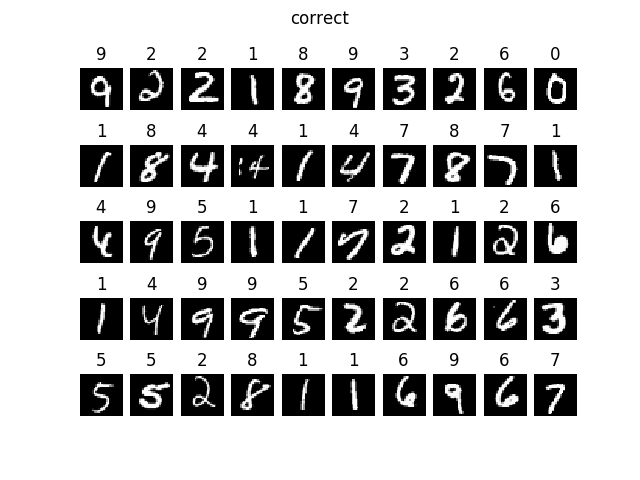
\includegraphics[clip, width=\linewidth]{../figures/result_assignment2_case1_correct.png}
		\subcaption{予測ラベルが実ラベルと一致したものの一例}
		\label{fig:case1_correct}
	\end{minipage}
	\begin{minipage}[b]{0.45\linewidth}
		\centering
		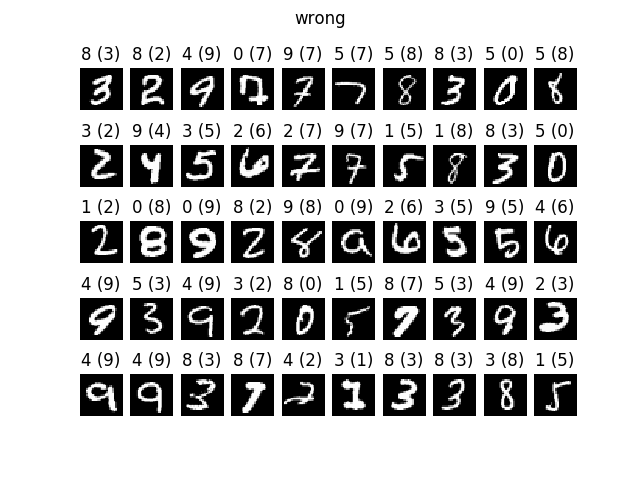
\includegraphics[clip, width=\linewidth]{../figures/result_assignment2_case1_wrong.png}
		\subcaption{予測ラベルが実ラベルと一致しなかったものの一例}
		\label{fig:case1_wrong}
	\end{minipage}
	\caption{Case 1のモデルの識別結果において予測ラベルと実ラベルが一致したもの・しなかったものの一例}
	\label{fig:case1_result}
\end{figure}


\clearpage
\begin{table}
    \centering
    \caption{Case 2の混同行列}
    \begin{tabular}{|r|rrrrrrrrrr|} \hline
        & 0 & 1 & 2 & 3 & 4 & 5 & 6 & 7 & 8 & 9 \\ \hline
        0 & 940 & 0 & 0 & 4 & 2 & 13 & 9 & 1 & 10 & 1 \\
        1 & 0 & 1,092 & 4 & 4 & 2 & 3 & 3 & 0 & 27 & 0 \\
        2 & 15 & 32 & 815 & 35 & 21 & 5 & 37 & 9 & 57 & 6 \\
        3 & 5 & 6 & 25 & 881 & 4 & 27 & 3 & 15 & 28 & 16 \\
        4 & 0 & 12 & 6 & 0 & 890 & 2 & 7 & 1 & 11 & 53 \\
        5 & 8 & 8 & 4 & 45 & 12 & 736 & 15 & 10 & 36 & 18 \\
        6 & 12 & 8 & 11 & 0 & 25 & 29 & 857 & 0 & 16 & 0 \\
        7 & 2 & 31 & 15 & 9 & 22 & 2 & 0 & 860 & 4 & 83 \\
        8 & 7 & 27 & 7 & 26 & 20 & 53 & 9 & 5 & 795 & 25 \\
        9 & 9 & 7 & 1 & 13 & 62 & 6 & 0 & 40 & 12 & 859 \\
        \hline
    \end{tabular}
    \label{tab:confusion_matrix_case2}
\end{table}
\vspace*{3\baselineskip}
\begin{figure}
	\begin{minipage}[b]{0.45\linewidth}
		\centering
		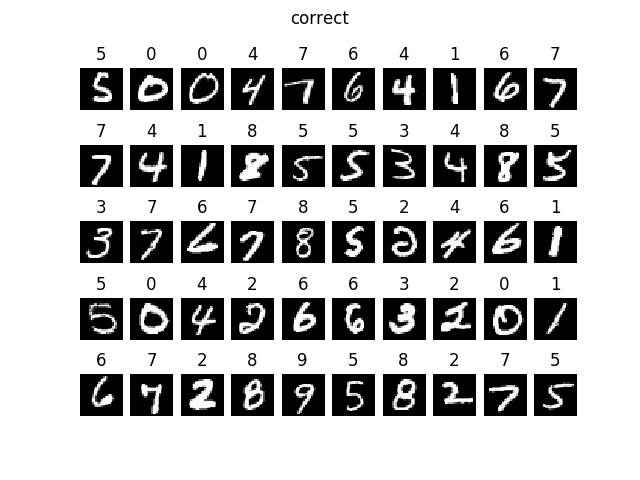
\includegraphics[clip, width=\linewidth]{../figures/result_assignment2_case2_correct.png}
		\subcaption{予測ラベルが実ラベルと一致したものの一例}
		\label{fig:case2_correct}
	\end{minipage}
	\begin{minipage}[b]{0.45\linewidth}
		\centering
		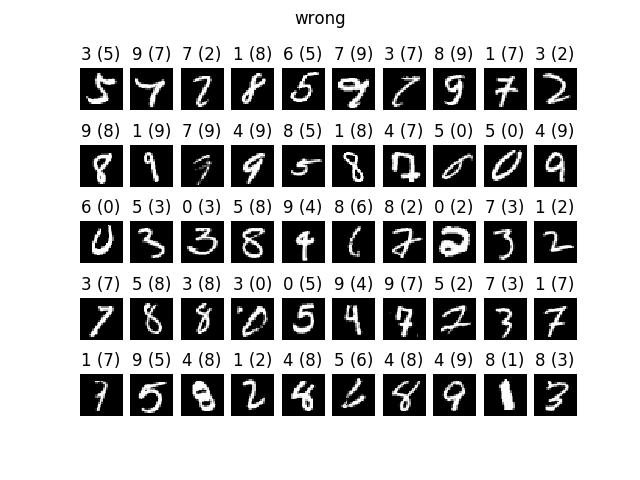
\includegraphics[clip, width=\linewidth]{../figures/result_assignment2_case2_wrong.png}
		\subcaption{予測ラベルが実ラベルと一致しなかったものの一例}
		\label{fig:case2_wrong}
	\end{minipage}
	\caption{Case 2のモデルの識別結果において予測ラベルと実ラベルが一致したもの・しなかったものの一例}
	\label{fig:case2_result}
\end{figure}


\clearpage
\begin{table}
    \centering
    \caption{Case 3の混同行列}
    \begin{tabular}{|r|rrrrrrrrrr|} \hline
        & 0 & 1 & 2 & 3 & 4 & 5 & 6 & 7 & 8 & 9 \\ \hline
        0 & 916 & 0 & 20 & 7 & 1 & 8 & 4 & 1 & 23 & 0 \\
        1 & 0 & 765 & 44 & 8 & 7 & 3 & 8 & 0 & 300 & 0 \\
        2 & 8 & 0 & 966 & 18 & 4 & 0 & 2 & 3 & 31 & 0 \\
        3 & 4 & 0 & 46 & 884 & 2 & 12 & 0 & 6 & 52 & 4 \\
        4 & 2 & 0 & 38 & 3 & 893 & 3 & 2 & 7 & 27 & 7 \\
        5 & 10 & 0 & 16 & 56 & 5 & 713 & 6 & 2 & 80 & 4 \\
        6 & 15 & 0 & 29 & 1 & 5 & 24 & 853 & 0 & 31 & 0 \\
        7 & 0 & 0 & 16 & 16 & 30 & 2 & 0 & 888 & 30 & 46 \\
        8 & 8 & 0 & 33 & 34 & 5 & 19 & 1 & 6 & 865 & 3 \\
        9 & 8 & 0 & 9 & 12 & 61 & 1 & 0 & 35 & 54 & 829 \\
        \hline
    \end{tabular}
    \label{tab:confusion_matrix_case3}
\end{table}
\vspace*{3\baselineskip}
\begin{figure}
	\begin{minipage}[b]{0.45\linewidth}
		\centering
		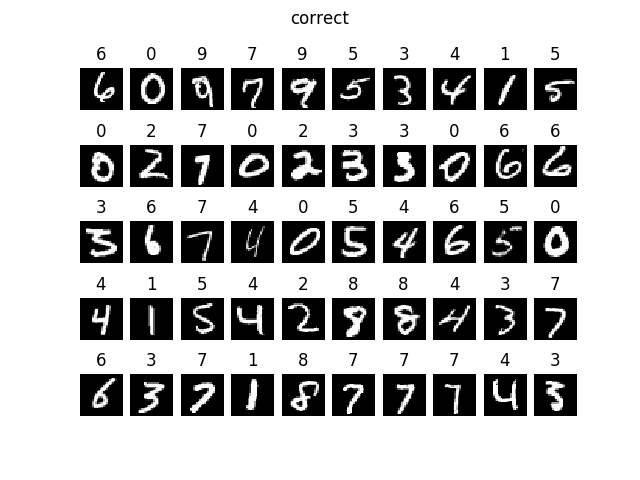
\includegraphics[clip, width=\linewidth]{../figures/result_assignment2_case3_correct.png}
		\subcaption{予測ラベルが実ラベルと一致したものの一例}
		\label{fig:case3_correct}
	\end{minipage}
	\begin{minipage}[b]{0.45\linewidth}
		\centering
		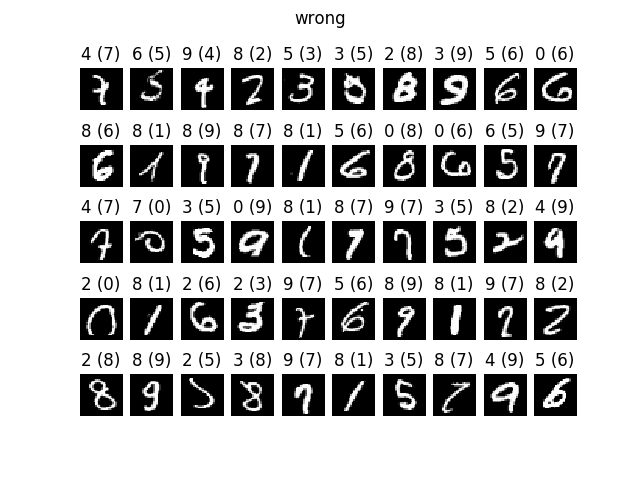
\includegraphics[clip, width=\linewidth]{../figures/result_assignment2_case3_wrong.png}
		\subcaption{予測ラベルが実ラベルと一致しなかったものの一例}
		\label{fig:case3_wrong}
	\end{minipage}
	\caption{Case 3のモデルの識別結果において予測ラベルと実ラベルが一致したもの・しなかったものの一例}
	\label{fig:case3_result}
\end{figure}



\clearpage
\subsection*{考察}

Case 2ではCase 1より全てのラベルで精度が高くなった。
これは,共分散行列のパラメータが1から\num{784 x 784}まで増えており,
モデルの表現力が高くなったためであると考えられる。
なお,Case 1のように全てのピクセルについて同じ分散を仮定するのは,
画像の端では値が0であることがほとんどであるのに対し
画像の中心部ではそうでないことが多いことから考えても,
モデルの表現力を制限しすぎていると考えられる。
一方,Case 2よりも\num{784 x 784 x 9}だけパラメータが多くなっているCase 3のモデルは,
Case 2よりも(全体での)精度が低くなってしまっている。
表\ref{tab:result}を見ると,
ラベル2と8の精度は大きく向上しているが,
特にラベル1の精度が30{\%}近く落ちてしまっている。
この原因として考えられることとしては,
trainデータの共分散行列がtestデータにおけるそれと大きくずれてしまっている可能性が挙げられる。


\end{document}
